% - ``Multi-Armed Bandit Learning in IoT Networks and non-stationary settings'', see https://hal.inria.fr/hal-01575419

\graphicspath{{2-Chapters/4-Chapter/CrownCom_17.git/}}

As explained before in Chapter~\ref{chapter:1}, the future IoT networks will require to support more and more communicating devices.
In this section, we show that intelligent devices in unlicensed bands can use MAB learning algorithms to improve spectral resource exploitation.
%
We evaluate the performance of two classical MAB learning algorithms, \UCB{} and Thomson Sampling, to handle the decentralized decision-making of Spectrum Access, applied to IoT networks.
We mean by \emph{decentralized} that learning is performed on the device side, and is spread on the totality of the devices in a network.
We also evaluate the learning performance when the number of intelligent end-devices grows.
%
We show that using learning algorithms
firstly extends devices battery autonomy (by reducing the packet-loss-ratio or equivalently, by improving the successful-communication rate),
and secondly does help to fit more devices in such networks, even when all end-devices are intelligent and are dynamically switching from channel to channel.
In the studied settings, stochastic MAB learning
% provides an up to $16\%$ gain in terms of successful transmission probabilities, and
has near optimal performance even in non-stationary settings with a majority of intelligent devices.

% \TODOL{Based on the publication, ``Multi-Armed Bandit Learning in IoT Networks and non-stationary settings'', see https://hal.inria.fr/hal-01575419}


The aim of this section is to assess the potential gain of learning algorithms in IoT scenarios, even when the number of intelligent devices in the network increases,
and the network usage is more and more fluctuatating.
% and the stochastic hypothesis is more and more violated.
To do that, we suppose an IoT network made of two types of devices: \emph{static devices} that use only one channel (fixed in time), and \emph{dynamic devices} that can choose the channel for each of their transmissions. Static devices form an interfering traffic, which could be generated by devices using other standards as well.
Note that instead of assuming that each static device uses a fixed channel, we could also assume a looser hypothesis: if each static device uses a fixed sub-set of the $K$ channels, and a purely uniform random access in its set of considered channels, then \emph{in average} the observed occupancy of the $K$ channels can be modeled as if it were occupied by (more) static devices using only one channel. So our first hypothesis is actually not constraining.
We first evaluate the probability of collision if dynamic devices randomly select channels (that is, a naive approach), and if a centralized controller would optimally distribute all of them in the channels at the beginning of the scenario.
This second approach is ideal, but not realistic the most common situation of decentralized co-located IoT networks, and it is just used here as a reference.
Then, these three reference scenarios allow to evaluate the performance of bandit algorithms, such as \UCB{} and TS, in a decentralized network, in terms of successful communication rate, as it reflects the network efficiency.
We show that these algorithms have near-optimal performance, even when the proportion of end-devices increases and the interfering traffic from other devices becomes less and less stochastic, more and more fluctuating and unpredictable.


% \textbf{Outline.}
% %
% The rest of this section is organized as follows. The system model is introduced in Section~\ref{sub:41:systemModel}. The reference policies are described in \ref{sub:41:threeReferencePolicies}, and our proposed sequential learning policies are introduced in \ref{sub:41:sequentialPolicies}.
% Numerical results are presented in \ref{sub:41:numericalResults}.


% ------------------------------------------------------------------------
\subsection{System model and notations}\label{sub:41:systemModel}

We present our system model, which consists of one gateway and many IoT devices, using a frequency- and time- slotted protocol.

\textbf{One gateway and many devices.}
%
We consider the system model presented in Figure~\ref{fig:41:system_model1}, where a set of devices all sends uplink packets to a (unique) network gateway.
Messages can be sent in a fixed number $K\geq2$ of wireless channels,
that are assumed to be orthogonal, that is, a message in channel $k$ will not cause collision to a message in another channel $j \neq k$.
% (\eg, $K=4$ or $K=16$ for instance), which are centered indifferently around the $433.5\;\mathrm{MHz}$ or the $877\;\mathrm{MHz}$ ISM bands (as it is chosen for the implementation presented in Section~\ref{sec:4:gnuradio}).
The communication between IoT devices and this gateway is done through a simple pure acknowledged ALOHA-based protocol where devices transmit uplink packets of fixed duration whenever they want.
We mean here by ALOHA-based that \emph{devices do not use sensing}, and \emph{we do not consider retransmissions of packets} (we relax this hypothesis in Section~\ref{sec:4:retransmissions}).
%
% Note that this choice of number of channels and of frequency bands is for instance the one of the current LoRa standard in Europe, but of course the precise choice does not really matter, and future standards can choose different parameters.

\begin{figure}[!t]
    \centering
    \includegraphics[width=0.70\linewidth]{system_model1.eps}
    \caption[In our system model, some dynamic devices (in the IoT network) transmit packets to a gateway and suffer from the interference generated by neighboring networks.]{In our system model, some dynamic devices (in the \textcolor{blue}{IoT network in blue}) transmit packets to a gateway and suffer from the interference generated by neighboring networks (in \textcolor{orange}{orange} left/right).}
    \label{fig:41:system_model1}
\end{figure}

The devices can transmit their packets in one of the $K$ channels. In the case where the gateway --of the corresponding IoT network-- receives an uplink message in one channel, it transmits an acknowledgement to the end-device in the same channel, after a fixed delay.
This is realistic in IoT networks such as networks based on LoRaWAN.
% (of $1\;\mathrm{s}$ in our implementation).
In a more general setting, if there were more than one gateway in the same IoT network being considered, the network would reply to the device by letting only one gateway sends back an acknowledgement.
The natural choice is for the network to send this acknowledgement by the gateway which received the uplink message.
For simplicity but without loss of generality, we consider a network with only one gateway,
but still it is important to observe the distinction between the gateway, which is simply a RF node, and the IoT network in charge of receiving, handling, and replying to the incoming uplink messages from the IoT devices being paired in the network.
%

These communications operate in unlicensed ISM bands and, consequently, they can suffer from interference generated by uncoordinated co-localized and/or neighboring networks (two are shown in \textcolor{orange}{orange} in Figure~\ref{fig:41:system_model1}, in left or right).
This interfering traffic is uncontrolled, and is most likely unevenly distributed over the $K$ different channels,
as each IoT protocol or IoT networks can choose to use a different subset of channels.
%
In order to simulate networks designed for the IoT, we consider a protocol \textbf{with no sensing} and no repetition of uplink messages. The gateway is in charge of sending back an acknowledgement, after some fixed-time delay, to any device paired with this gateway in this network (\ie, in \textcolor{blue}{blue} in Figure~\ref{fig:41:system_model1}) who succeeded in sending an uplink packet.
%
By considering a small number of orthogonal wireless channels, and a unique PHY layer configuration (\ie, modulation, waveform, etc), and in case of a non-uniform traffic in the different channels,
the device can improve their usage of the network if they are able to \emph{learn} on the fly the best channels to use, that is, the most vacant one. Indeed, in this model, the \emph{quality} of the channels (\ie, the ressources) are identified by their vacancy, or one minus their occupancy rates.

We note that MAB learning has also started to be applied to also optimize the PHY layer parameters, see for instance \cite{KerkoucheAlami18} following our article \cite{Bonnefoi17},
but in this thesis we chose to restrict to the spectrum access problem and thus we only MAB models where the arms correspond to orthogonal frequency bands.


\paragraph{Slotted protocol.}
%
For simplicity, and for consistency with the rest of this thesis, we only consider a discrete protocol (\ie, slotted).
As illustrated in Figure~\ref{fig:41:protocol}, we suppose a slotted protocol, in both time and frequency.
All devices share a synchronized time, and know in advance $K$, the finite number of available RF channels.
In each time slot, the devices try to send packets to the unique gateway, which listens continuously to all channels, following an ALOHA-based communication, with no sensing.
Each time slot is divided in two parts: first for uplink communications in which data packets are sent by end-devices to the gateway.
In one channel, if only one packet is sent in this part of the slot, the gateway can decode it and sends an acknowledgement to the device in the second part (on the same channel).
If two or more devices send an uplink packet in the same slot, the uplink packets collide, and the acknowledgement (\Ack) is not transmitted. In this case, we say that there is a \emph{collision} in this time slot.
In other words, if the gateway cannot successfully decode the incoming (uplink) messages because they were corrupted by collisions, it does not send any \Ack{} back.
This way, no collision can occur on the downlink messages, easing the analysis of collisions.

\begin{figure}[!h]
    \centering
    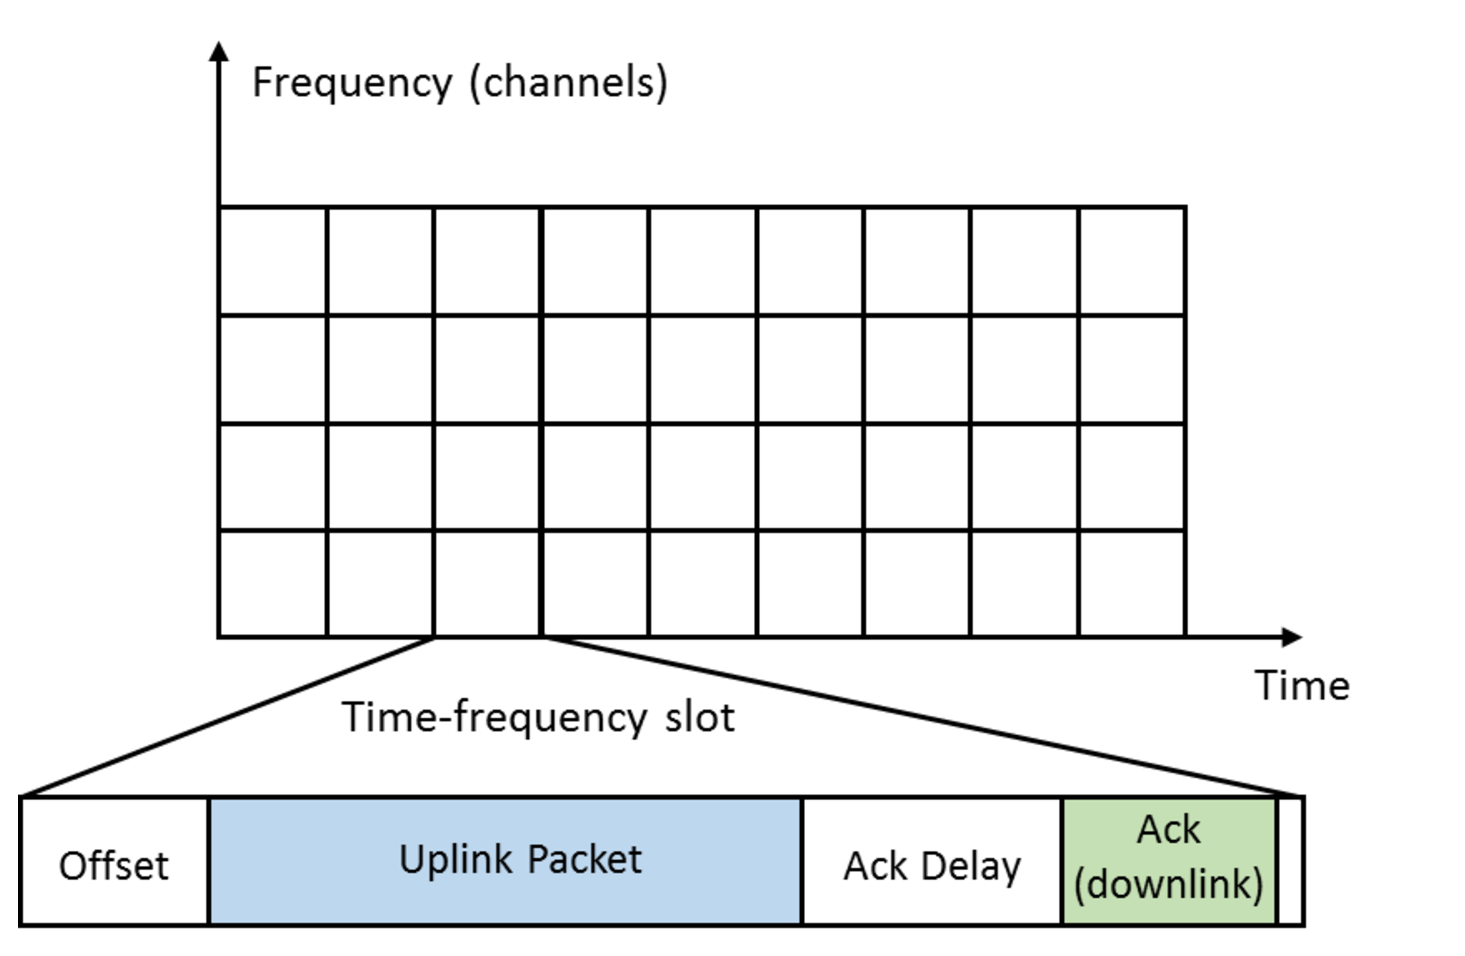
\includegraphics[scale=0.40]{protocol.eps}
    \caption[The considered time-frequency slotted protocol. Each frame is composed by a fixed duration uplink slot in which the end-devices transmit their (uplink) packets. If a packet is well received, the gateway replies by transmitting an \Ack, after the ack delay.]{The considered time-frequency slotted protocol. Each frame is composed by a fixed duration \textcolor{blue}{uplink slot} in which the end-devices transmit their \textcolor{blue}{(uplink) packets}. If a packet is well received, the gateway replies by transmitting an \textcolor{darkgreen}{\Ack}, after the ack delay.}
    \label{fig:41:protocol}
\end{figure}


\paragraph{Static vs dynamic devices.}
%
We make the following assumptions on the network.
We assume that there are two types of end-devices in the network:
\begin{itemize}
    \item
    \emph{Static} end-devices are identical, and each of them uses only \emph{one} channel to communicate with the gateway, with no loss of generality.
    %  if devices random access the channels.
    Their choice is assumed to be fixed in time (\ie, stationary). The traffic generated by these devices is considered as an interfering traffic for other devices.
    \item
    \emph{Dynamic} (or \emph{smart}) end-devices can use all the available channels, by quickly changing their communication channel at any time slot, following a Machine Learning policy.
    For that end, they use their history of past communication successes or failures they experienced in each channel, to learn about channel availability.
    We also assume that the dynamic end-devices can run simple embedded decision making algorithms, and have limited but reasonable computing as well as storage capacities.
    Note that of course we assume a limited storage capacity, so no device stores the full history of communication successes and failures, but they only store average rates (which can be stored using one float number for each of the $K$ channels).
    Our goal is to propose a learning algorithm than can be implemented by each dynamic device, in a decentralized and independent manner, in order to improve their successful communication rate automatically.
\end{itemize}

We further assume that there are $K \geq 2$ channels, $D \geq 0$ dynamic end-devices, and $S \geq 0$ static devices
with $0 \leq S_k \leq S$ static devices in channel $k \in [K]$ (so $S = \sum_{k=1}^{K} S_k$).


\textbf{Random emission patterns:}
%
We suppose that all devices follow the same emission pattern, being fixed in time, and we choose to model it as a simple Bernoulli process:
all devices have the same probability to send a packet in any (discrete) temporal slot, and we denote $p \in (0, 1)$ this probability\footnote{~In the experiments below, $p$ is about $10^{-3}$, because in a crowded network $p$ should be smaller than $K / (S + D)$ for all devices to communicate successfully (in average).}.
The parameter $p$ essentially controls the frequency of communication for each device, once the time scale is fixed, and $1/p$ is proportional to the \emph{duty cycle}.
% (\ie, real time during two messages)
For instance, for IoT devices sending messages with a duration of $1$ second and possibly at every second, then on a daily basis we have $p = 1 / (12 \times 60 \times 60) \simeq 1.5 \times 10^{-5}$.


\textbf{Some assumptions on the network occupation:}
%
We focus on \emph{dense networks}, in which the number of devices $S + D$ is very large compared to $K$ (for instance, about $1000$ to $100000$, while $K$ is about $4$ to $256$).
As this problem is only interesting if devices are able to communicate reasonably efficiently with the gateway, we assume that devices only communicate occasionally, \ie, with a low \emph{duty cycle}, as it is always considered for IoT.
Note that even unlicensed bands have such limitations, as for instance this is a strict requirement for any device using the \SI{868}{\mega\hertz} ISM band in Europe (and its regulation also enforces a maximum transmission power, but we do not consider power transmission in this work).
%
We prefer this choice rather than non-crowded networks, \ie, where $S + D \leq K$, as the former makes more sense for realistic IoT networks.\\
% \footnote{~Here, $K$ will typically be about $10$ different radio channels, usually in the same RF band and with separate mean carrier frequencies, and the number of devices will be of the order of $1000$ to $10000$.}.
\indent
On the opposite, imagine if there were only $K=4$ channels being occupied by $D+S = 100$ devices, each communicating with a high rate of $p=1/10$, with a non-zero occupancy in each channel (\ie, $\forall k, S_k > 0$). Then, almost all time slots will lead to collisions in all channels, for a uniformly random access scheme, and thus the network efficiency (\ie, successful communication rate) will be so close to zero that using learning algorithms cannot improve much.
Such scenario is not our target of interest, and thus we prefer to only consider feasible scenarios where $p$ is smaller than $K/(S+D)$, in order to \emph{have an average of active devices not larger\footnote{~In Chapter~\ref{chapter:5} we simply consider the case of $p=1$ and $M = D \leq K$ dynamic devices, referred to as \emph{players}.} than the number of channels}.


\textbf{Link with the MAB model:}
%
All devices follow a Bernoulli emission process.
Consider the network from the point of view of one dynamic device:
every time a dynamic device has to communicate with the gateway,
it has to choose one channel (at each transmission $t \geq 1, t \in \mathbb{N}$), denoted as $A(t) = k \in[K]$.
Then, the dynamic device waits in this channel $A(t)$ for an acknowledgement sent by the gateway, during a certain period (\eg, $5$ seconds for the example considered above).
Before sending another message (\ie, at time $t+1$), the dynamic device knows if it received or not this \Ack{} message.
%
For this reason, selecting channel (or arm) $k$ at time $t$ yields a (random) feedback, called a (binary) \emph{reward}, $r(t) \eqdef Y_{k,t} \in \{0,1\}$, being $0$ if no \Ack{} was received before the next message, or $1$ if \Ack{} was successfully received.
The goal of the dynamic device is to minimize its packet loss ratio, or equivalently, to maximize its number of successful transmissions, or its cumulative reward,
$\sum_{t = 1}^T r(t),$
which is the usual objective in MAB problems (see Section~\ref{sec:2:notations}).


This problem is a special case of the stochastic MAB with
% , where the sequence of rewards drawn from a given arm $k$ is assumed to be  \emph{i.i.d.}, under some distribution $\nu_k$, that has a mean $\mu_k$.
% Several types of reward distributions have been considered in the literature, and rewards are binary in our model.
% We consider only
Bernoulli distributions.
% , in which $r_k(t) \sim \mathrm{Bern}(\mu_k)$, that is, $r_k(t) \in \{0,1\}$ and $\mathbb{P}(r_k(t) = 1) = \mu_k \in [0,1]$.
Contrarily to many previous work done in the CR field and for Opportunistic Spectrum Access \cite{Jouini10,Jouini12},
the reward $r(t)$ does \emph{not} come from a sensing phase before sending the $t$-th message, as it would do for any ``listen-before-talk'' model.
In our model, rewards rather come from receiving or not an acknowledgement from the gateway, between the $t$-th and $t+1$-th messages. A reward of one indicates that the acknowledgement was received on time, and a reward of zero indicates the opposite.

The problem parameters
% are $\mu_1,\dots,\mu_K$, the mean availability of the channels,
are $S_1, \dots, S_K$ which represent the (stationary) occupancy of the channels by the static devices,
and they are unknown to each dynamic device, so to maximize their cumulated rewards, they must learn the distributions of the channels, in order to be able to progressively improve their respective successful communication rate.
%
The goal is thus to propose a simple sequential algorithm to be applied identically and independently by each dynamic device, in a fully distributed setting (each device runs its own algorithm, from its observations), in order to minimize collisions and maximize the fraction of successful transmissions of all the dynamic devices.
%
This requires to tackle the so-called \emph{exploration-exploitation dilemma}: a device has to try all channels a sufficient number of times to get a robust estimate of their qualities, while not selecting the worst channels too many times.
%
Before presenting the MAB algorithms used in the experiments, we present some simple baseline (reference) policies.


% ------------------------------------------------------------------------
\subsection{Three reference policies}\label{sub:41:threeReferencePolicies}

We present three different policies that can be used to assess the efficiency of the learning algorithms presented later on.
The first one is naive but can be used in practice, while the two others are very efficient but require full knowledge on the system (\ie, an oracle) and are thus unpractical.
%
They are however useful for our numerical simulations, and are used as references, to show that our MAB-based approaches quickly learn to perform almost optimally.
%
Their short names are used in the legend on Figures~\ref{fig:41:from10to100}, \ref{fig:41:figure4appendix}), and are given in ``quotes'' in the corresponding paragraphs.


\paragraph{$1^{\text{st}}$ - Naive policy: Random Channel Selection} (``\textcolor{darkgreen}{Random}'')

We derive here the probability of having a successful transmission, for a dynamic device, in the case where all the dynamic devices make a purely random channel selection (\ie, uniform on $i \in [K]$).
This reflects a naive policy that could be implemented by all the dynamic devices, and it provides a reference scenario to compare against.
Note that even nowadays this is still the solution implemented for real IoT devices deployed in new LoRaWAN networks.

In this case, for one dynamic device, a successful transmission happens if it is the only device to choose channel $k$, at that time slot.
the $S_k$ static devices in each channel $k$ are assumed to be independent, and static and dynamic devices are assumed to \emph{not} transmit at each time $t$ with a fixed probability $1-p$,
so probability of successful transmission is computed as follows

\begin{equation}
    \Pr(\text{success}|\text{sent}) = \sum_{k=1}^{K} \underbrace{\Pr(\text{success}|\text{sent in channel}\;k)}_{\text{No one else sent in channel}\; k} \; \underbrace{\Pr(\text{sent in channel}\,k)}_{= 1/K, \text{ by uniform choice}}
\end{equation}

All dynamic devices follow the same policy in this case, so the probability of transmitting at that time in channel $k$ for any dynamic device is $p / K$, and there are $D-1$ other dynamic devices.
As they are independent, the probability that no other dynamic device sent in $i$
% $\Pr(\text{no other dynamic device sent in}\;i)$,
is $q = \Pr(\bigcap_{k=1}^{D-1} \text{device}\;k\;\text{did not sent in}\;i) = \prod_{k=1}^{D-1} \Pr(\text{device}\;k\;\text{did not sent in}\;i)$. And $\Pr(\text{device}\;k\;\text{sent in}\;i) = p \times 1 / K$, by uniform choice on channels and the Bernoulli emission hypothesis. So $q = \prod_{k=1}^{D-1} (1 - p/K) = (1-p/K)^{D-1}$. Thus we can conclude,
%
\begin{align}\label{eq:41:strategynaive}
    \Pr(\text{success}|\text{sent})
    & = \sum_{k=1}^{K} \underbrace{(1 - p / K)^{D-1}}_{\text{No other dynamic device}} \times \underbrace{(1-p)^{S_k}}_{\text{No static device}} \times\; \frac{1}{K} \nonumber \\
    & = \frac{1}{K} \left(1-\frac{p}{K}\right)^{D-1} \sum_{k=1}^{K} (1-p)^{S_k} .
\end{align}
%
This expression \eqref{eq:41:strategynaive} is constant (in time), and easy to compute numerically, but comparing the successful transmission rate of any policy against this naive policy is important, as any efficient learning algorithm should outperform it
(maybe after a long enough initial learning period).


\paragraph{$2^{\text{nd}}$ - (Unachievable) Optimal oracle policy} (``\textcolor{orange}{Optimal}'')

We investigate here the optimal policy that can be achieved if the dynamic devices have a perfect knowledge of the repartition of static devices $(S_k)_k$, and a fully centralized decision making\footnote{~This optimal policy needs an \emph{oracle} seeing the entire system, and affecting all the dynamic devices, once and for all, for a fixed stationary scenario, in order to avoid any signaling overhead. This is not possible in IoT contexts as several completely independent networks may operate in a single place.} is possible.
We want to find the stationary repartition of devices into channels that maximizes the probability of having a successful transmission.

If the oracle chooses a fixed configuration of dynamic devices, it means that for each dynamic device the oracle affects it to a unique channel for all time steps.
Then there is a number $D_k$ of devices affected to channel $k$ being fixed in time (\ie, stationary),
and thus this probability is computed as before:
%
\begin{align}\label{eq:41:prob_col}
    \Pr(\text{success}|\text{sent})
    & = \sum_{k=1}^{K} \Pr(\text{success}|\text{sent in channel}\;k) \; \Pr(\text{sent in channel}\;k) \nonumber \\
    & = \sum_{k=1}^{K} \underbrace{(1 - p)^{D_k - 1}}_{\;\;D_k - 1 \;\text{others}\;\;} \times \underbrace{(1 - p)^{S_k}}_{\;\;\text{No static device}\;\;} \times \underbrace{ D_k / D }_{\;\;\text{Sent in channel}\; k\;\;}.
\end{align}

Consequently, an optimal allocation vector $(D_1,\dots,D_{K})$ is a solution of the following real-valued constraint optimization problem:
%
\begin{subequations}\label{eq:41:prob}
\begin{align}
    % \begin{cases}
    \underset{D_1,\dots,D_{K}}{\arg\max}\; & \sum_{k=1}^{K} D_k (1 - p)^{S_k + D_k -1}, \label{eq:41:optPb}\\
    \text{such that}\;\; & \sum_{k=1}^{K} D_k = D, \label{eq:41:eqCstr}\\
    & D_k \geq 0 \qquad \forall k\in\llbracket 1;K\rrbracket . \label{eq:41:ineqCstr}
    % \end{cases}
\end{align}
\end{subequations}

\begin{proposition}\label{prop:41:Lagrangian}
\begin{leftbar}[propositionbar]  % XXX leftbar propositionbar, comment if needed
    The \emph{Lagrange multipliers} method \cite{BoydVanderberghe04} can be used to solve the constraint real-valued maximization problem introduced in equation \eqref{eq:41:prob}.
    %
    It gives a closed form expression for the (unique) optimal solution $D_k^*(\lambda)$, depending on the system parameters, and the unknown Lagrange multiplier $\lambda \in \mathbb{R}$.
    %
    \begin{equation}\label{eq:41:Dilambda}
        D_k^*(\lambda) = \left(\frac{1}{\log(1-p)}\left[ \mathcal{W}\left(\frac{\lambda \e}{(1-p)^{S_k-1}} \right)-1 \right]\right)^{+} .
    \end{equation}
\end{leftbar}  % XXX leftbar propositionbar, comment if needed
\end{proposition}
%
\begin{smallproof}
\begin{itemize}
    \item
    In a realistic scenario, we can assume that $D_k\leq \frac{-2}{\ln\left(1-p\right)} \approx \frac{2}{p},\quad \forall k\in\llbracket 1;K \rrbracket$. For such values for $D_k$, the objective function $f: (D_1, \dots, D_{K}) \mapsto \sum_{k=1}^{K} D_k (1 - p)^{S_k + D_k -1}$ is concave as the sum of concave functions
    \footnote{~It is worth noting that $f$ is neither concave nor quasi-concave on $[0,\infty)^{K}$ \cite{Luenberger68,Yaari77}.}.
    \item
    The Lagrange multipliers method can be applied to the optimization problem \eqref{eq:41:optPb}, with a concave objective function $f$, linear equality constraints \eqref{eq:41:eqCstr} and linear inequality constraints \eqref{eq:41:ineqCstr}. The strong duality condition is satisfied in this case \cite{BoydVanderberghe04}, so finding the saddle points will be enough to find the maximizers.
    % \item
    % \hfill{}$\square$
    \end{itemize}
    More details are given in Section~\ref{sec:4:proofLagrangian} in the Appendix of this Chapter.
\end{smallproof}

Where in the equation~\eqref{eq:41:Dilambda}, $(a)^{+} \eqdef \max(a,0)$, and $\mathcal{W}$ denotes the $\mathcal{W}$-Lambert function which is the reciprocal bijection of $x \mapsto x e^x$ on $\mathbb{R^+} = [0, +\infty)$ (which can be computed numerically in an efficient manner, \cite{Corless96}).
Moreover, condition \eqref{eq:41:eqCstr} implies that the Lagrange multiplier $\lambda$ is the solution of the constraint $\sum_{k=1}^{K} D_k^*(\lambda) = D$.
%
This single constraint can be solved numerically, with simple one-dimensional root finding algorithms.
Solving the optimization problem provides the optimal real number value for $D_k^*$, which has to be rounded\footnote{~Any rounding choice will give about the same repartition, up-to a difference of only one device by channel, and so we chose to round from below for the first channels.} to find the optimal number of devices for channel $k$:
%
$\widehat{D_k} = \lfloor D_k^* \rfloor$ for $1 \leq k < K$, and $\widehat{D_{K}} = D - \sum_{k=1}^{K - 1} \widehat{D_k}$.


\paragraph{$3^{\text{rd}}$ - A greedy approach of the oracle strategy} (``\textcolor{deeppurple}{Good sub-optimal}'')

We propose a \emph{sequential} approximation of the optimal policy:
the third solution is a sub-optimal naive policy, simple to set up, but also unpractical as it also needs an oracle.
End-devices are iteratively inserted in the channels with the lowest load (\ie, the index $k$ minimizing $S_k + D_k(\tau)$ at global time step $\tau$). Once the number of devices in each channel is computed, the probability of sending successfully a message is also given by equation \eqref{eq:41:prob_col}.
This is the policy that would be used by dynamic devices if they were inserted one after the other, and if they had a perfect knowledge of the channel loads.


% ----------------------------------------------------------------------
\subsection{Sequential policies based on bandit algorithms}
\label{sub:41:sequentialPolicies}
% ----------------------------------------------------------------------

While the stochastic MAB model has been used to describe some aspects of Cognitive Radio systems, it is in principle not suitable for our IoT model, due to the non-stationarity of the channels occupancy, caused partly by the learning policy used by dynamic devices, but mainly by their random activation processes.
%
In our model, every dynamic device implements its own learning algorithm, \emph{independently}.
For one device, the time $t$ refers to the number of time it accessed the network (following its Bernoulli transmission process, \ie, its duty cycle), \emph{not} the total number of time slots from the beginning, as rewards are only obtained after a transmission, and IoT devices only transmit sporadically, due to low transmission duty cycles.


\textbf{Using a bandit algorithm for IoT devices:}
%
Our IoT application is challenging in that there are \emph{multiple} players (the dynamic devices) interacting with the \emph{same} arms (the channels), without any centralized communication (they do not even know the total number of dynamic devices).
%
% Considered alone, each dynamic device
We propose algorithms in which each dynamic device ignores all the other one and
implements a learning algorithm to play a bandit game.
%
In each time slot, if it has to communicate (which happens with probability $p$), then it chooses a channel and it receives a reward $1$ if the transmission is successful, $0$ otherwise.
Each device aims at maximizing the sum of the rewards collected during its communication instants, which shall indeed maximize the fraction of successful transmissions. Besides the modified time scale (rewards are no longer collected at every time step), this looks like a usual bandit problem.
However, it cannot be modeled as a stochastic MAB, as the rewards are (unfortunately) \emph{not} \iid: they not only depend on the (stationary, \iid) behavior of the static devices, but also on the behavior of other dynamic devices, that is not stationary (because of learning and random activation of each device).
%
Despite this, we show in the next subsection that running a stochastic bandit algorithm for each device based on its own rewards is surprisingly successful.


\textbf{Considered algorithms.}
%
% In our model, every dynamic device implements its own algorithm, \emph{independently}.
% For one dynamic device, the time $t$ is the total number of sent messages from the beginning, as rewards are only obtained after a transmission.
%
The two algorithms we consider are \UCB{} (``\textcolor{blue}{UCB}'' in the figures)
and Thompson sampling (TS) (``\textcolor{red}{Thompson-sampling}''),
and they are presented in Section~\ref{sec:2:famousMABalgorithms}.
% originally $\alpha$ was set to $2$ \cite{Auer02}, but empirically $\alpha = 1/2$ is known to work better (uniformly across problems), and $\alpha > 1/2$ is advised by the theory \cite{Bubeck12}.
%
The \UCB{} algorithm uses $\alpha = 1/2$ in our experiments.
The TS algorithm is known to be empirically efficient, and for these reasons it has been used successfully in various applications, including problems from Cognitive Radio \cite{Toldov16,Mitton16}, and also in previous work on decentralized IoT-like networks \cite{Darak16}.
% although being simple and easy to implement, is known to perform well for stochastic problems, for which it was proven to be asymptotically optimal \cite{AgrawalGoyal11,Kaufmann12Thompson}.


\textbf{\emph{Adversarial} bandit algorithms?}
%
Instead of using MAB algorithms assuming a stochastic hypothesis on the system, we could try to use MAB algorithms designed to tackle a more general problem, that makes no hypothesis on the interfering traffic.
The \emph{adversarial MAB} algorithms is a broader family, of which a well-known and efficient example is the $\mathrm{Exp}3$ algorithm \cite{Auer02,Bubeck12}.
Empirically, the $\mathrm{Exp}3$ algorithm turned out to perform significantly worse than both \UCB{} and TS in the same experiments,
therefore we did not report results here.
% % FIXME maybe we should... ?
% %(see Section \ref{sub:41:numericalResults}).
% However, contrarily to the two stochastic algorithms, the use of $\mathrm{Exp}3$ is correctly justified, even in the non-stationary model, as its performance guarantees are true in \emph{any} setting.
% But it is not so surprising that it performs worse, as the theoretical performance guarantees of adversarial MAB algorithms are an order of magnitude
% %\footnote{~We preferred not to talk about \emph{regret} in this study, but in a few words: it is a measure of how \emph{bad} the algorithm performed in terms of its accumulated rewards, in comparison to the best possible policy, and should be as small as possible. For stochastic algorithms, being ``efficient'' means having a regret bounded as $R_T = \mathcal{O}(\log T)$, but for adversarial algorithms, it means having $R_T = \mathcal{O}(\sqrt{K T})$.}
% worse than the one for stochastic ones.
% (in their respective case of application).
% Further research on this aspect could lead to interesting future works.



% ------------------------------------------------------------------------
\subsection{Numerical results}\label{sub:41:numericalResults}

% Simulation parameters
We suppose a network with $S + D = 2000$ end-devices, and one IoT gateway.
Each device sends packets following a Bernoulli process, of probability $p = 10^{-3}$ (\eg, this is realistic: one packet sent about every $20$ minutes, for time slots of $1\mathrm{s}$).
The RF band is divided in $K = 10$ channels.
Each static device only uses one channel, and their uneven repartition in the $10$ channels is chosen as $(S_1,\cdots, S_{K}) = S \times (0.3, \, 0.2, \, 0.1, \, 0.1, \, 0.05, \, 0.05, \, 0.02, \, 0.08, \, 0.01,$ $0.09)$, to keep the same proportions when $S$ decreases. The dynamic devices have access to all the channels, and use learning algorithms.
%to find the least loaded.
%
We simulate the network during $10^6$ discrete time slots, during which each device transmits on average $1000$ packets (\ie, the learning time is about $1000$ steps, for each algorithm).
We tried similar experiments with other values for $K$ and this repartition vector, and results were similar for non-homogeneous repartitions.

Clearly, the problem is less interesting for a homogeneous repartition, as all channels appear the same for dynamic devices, and so even with $D$ small in comparison to $S$, the system behaves like in Figure~\ref{fig:41:100intelligent}, where the performance of the five approaches are very close.

\begin{figure}[!h]
    \centering
    \subfloat[][10\% of dynamic devices]{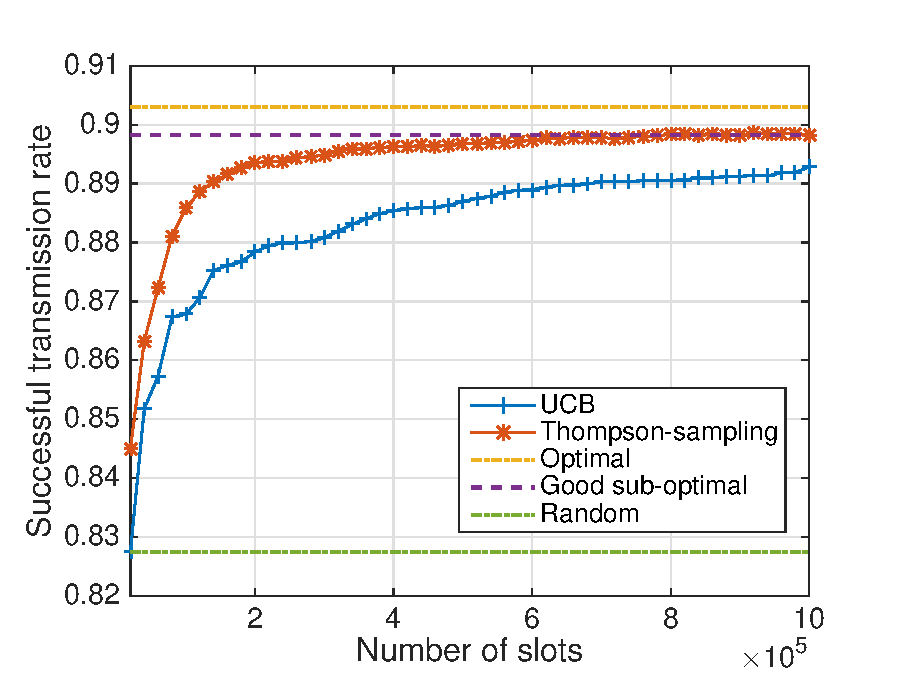
\includegraphics[width=0.52\textwidth]{10intelligent.eps}
    \label{fig:41:10intelligent}}
    %
    \subfloat[][30\% of dynamic devices]{\includegraphics[width=0.52\textwidth]{30intelligent.eps}
    \label{fig:41:30intelligent}}
    %
    \vspace*{-10pt}
    \subfloat[][50\% of dynamic devices]{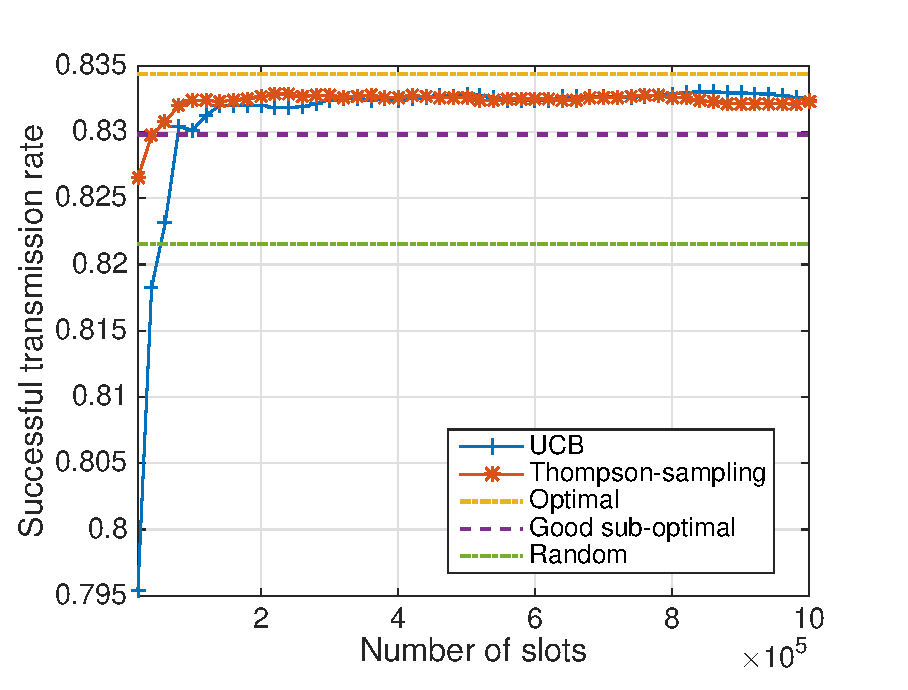
\includegraphics[width=0.52\textwidth]{50intelligent.eps}
    \label{fig:41:50intelligent}}
    %
    \subfloat[][100\% of dynamic devices]{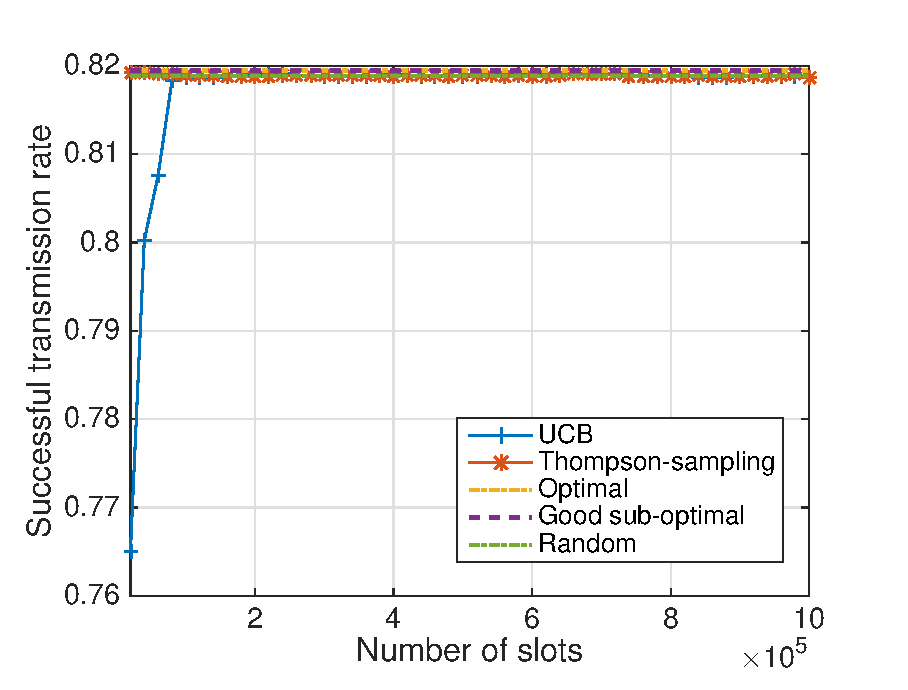
\includegraphics[width=0.52\textwidth]{100intelligent.eps}
    \label{fig:41:100intelligent}}
    \caption{Performance of two MAB algorithms (\UCB{} and Thompson Sampling), compared to extreme reference policies without learning or oracle knowledge, when the proportion of dynamic end-devices in the network increases, from $10\%$ to $100\%$.}
    \label{fig:41:from10to100}
    \vspace*{-10pt}
\end{figure}


\paragraph{First results.}
%
Figure~\ref{fig:41:from10to100} presents the successful transmission rate as a function of time.
The two MAB algorithms, \UCB{} and Thompson Sampling (TS), are compared against the naive random policy (which are outperformed easily by the MAB algorithms), and the two (optimal and greedy) oracle policies (which outperform slightly the MAB algorithms).
The results are displayed when $10\%$, $30\%$, $50\%$ and $100\%$ of the traffic is generated by dynamic devices.


We can see in Figure~\ref{fig:41:from10to100} that the TS algorithm (\textcolor{red}{in red}) outperforms the \UCB{} algorithm (\textcolor{blue}{in blue}), when the number of end-devices is below 50\%. When the number of end-devices is higher, both algorithms have almost the same performance, and perform well after a small number of transmissions (\ie, they show quick convergence).
Moreover, we can see in Figures~\ref{fig:41:10intelligent}, \ref{fig:41:30intelligent}, and \ref{fig:41:50intelligent} that both have better success rate than the random policy and the probability of successful transmission is between the optimal oracle and suboptimal oracle policies.
For instance, for $10\%$ of dynamic devices, after about $1000$ transmissions, using \UCB{} over the naive uniform policy improved the successful transmission rate from $83\%$ to $88\%$, and using Thompson Sampling improved it to $89\%$.
Increasing the number of end-devices decreases the gap between the optimal and random policies:
as expected intuitively, the more dynamic devices, the less useful are learning algorithms, and basically for networks with only dynamic devices, the random policy is as efficient as the optimal one, as seen in Figures~\ref{fig:41:100intelligent} and on the right end side of Figure~\ref{fig:41:perf_learning}.

\begin{figure}[!h]
    \centering
    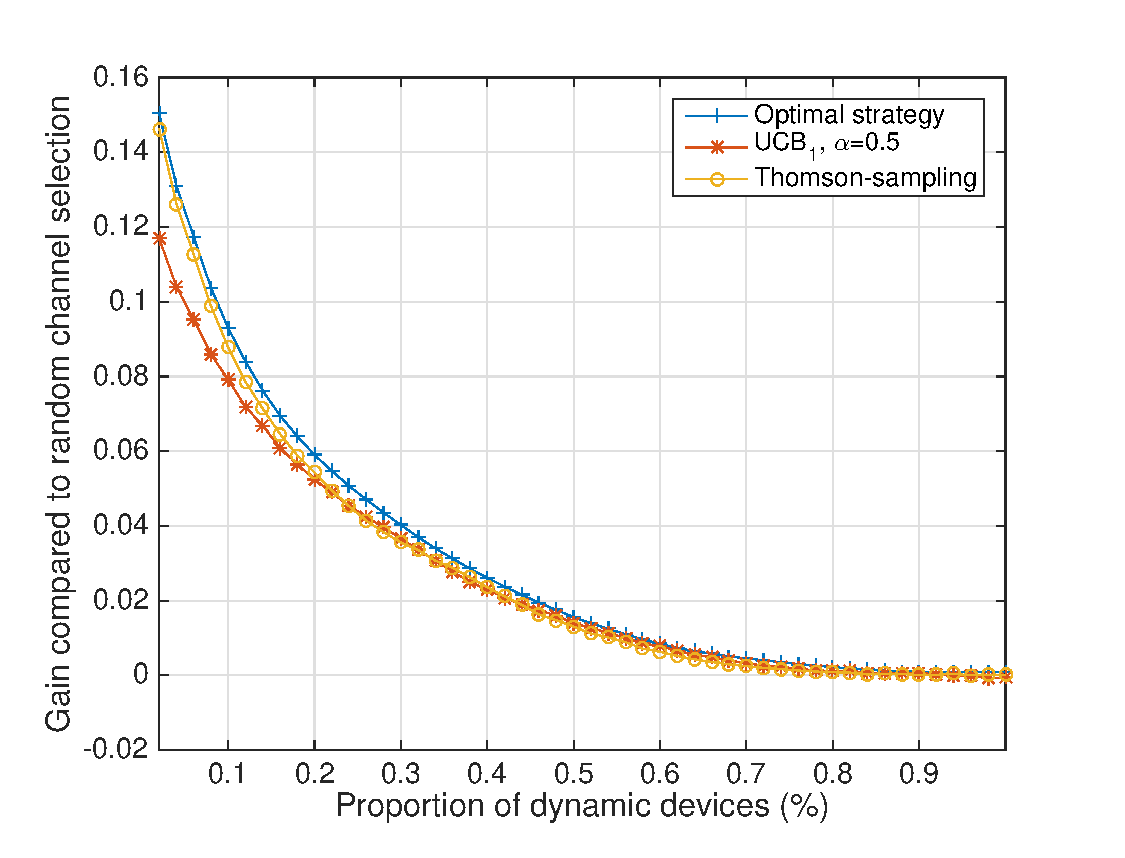
\includegraphics[scale=0.65]{perf_learning.eps}
    \caption{Learning with \UCB{} and Thomson Sampling, with many dynamic devices.
        The learning gain, for each device, decreases with the proportion of dynamic devices in the network.
        Note that the values ($16\%$ etc) depend on the repartition of static devices into the $K$ channels (\ie, $S_1,\dots,S_K$) but the general profile of this plot does \emph{not} depend much on these parameters.
        % Both algorithms achieve close to optimal performance after a reasonable learning time.
    }
    \label{fig:41:perf_learning}
\end{figure}


\textbf{Successful transmission rate as a function of the number of dynamic devices.}
%
To better assess the evolution of the optimal policy compared to the random one, we have displayed on Figure~\ref{fig:41:perf_learning} the evolution of the gain, in terms of successful transmission rate, provided by the optimal oracle and the two learning policies, after $10^6$ time slots, \ie, about $1000$ transmissions for each IoT device.
We can see that when the proportion of end-devices is low (\eg, $1\%$ of devices are dynamic), the optimal policy provides an improvement of $16\%$ compared to random channel selection.
The TS algorithm always provides near-optimal performance, but the \UCB{} algorithm has a lowest rate of convergence and performs consequently worse after $1000$ transmissions, for instance it only provides a gain of $12\%$ for the same proportion of dynamic devices ($1\%$),
for the considered values of $S_1,\dots,S_K$.

\begin{figure}[!h]
    \centering
    \subfloat[][10\% of intelligent devices]{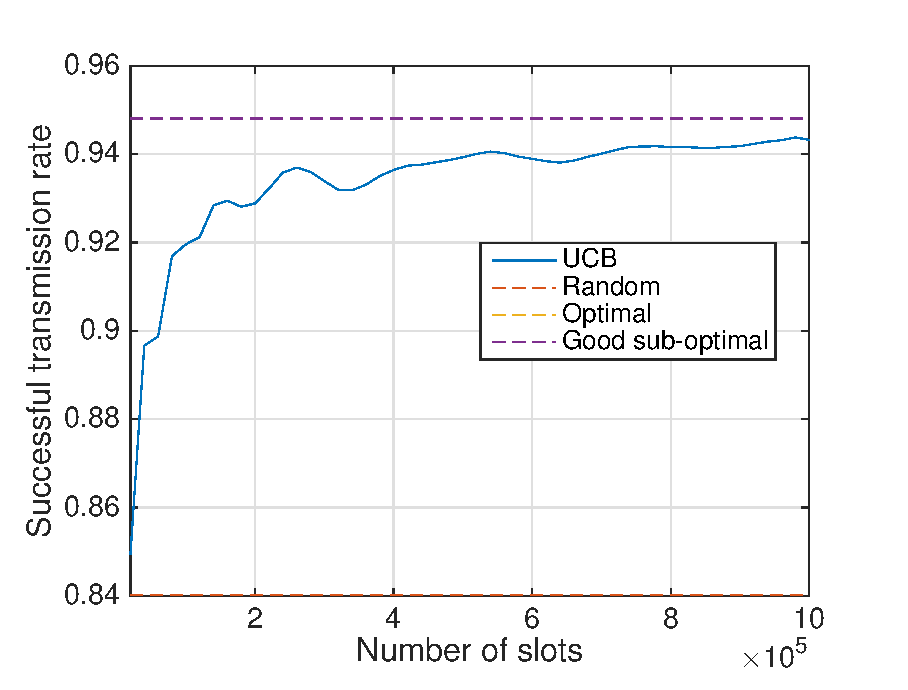
\includegraphics[width=0.47\textwidth]{ch2_10.eps}
    \label{fig:41:ch2_10}}
    %
    \subfloat[][30\% of intelligent devices]{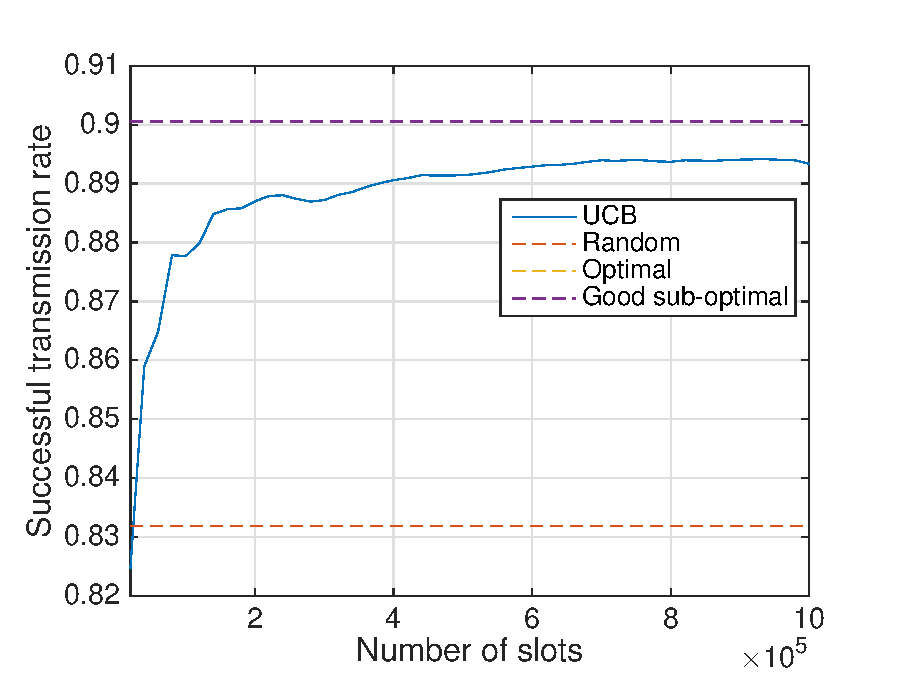
\includegraphics[width=0.47\textwidth]{ch2_30.eps}
    \label{fig:41:ch2_30}}
    %
    \vspace*{-10pt}
    \subfloat[][50\% of intelligent devices]{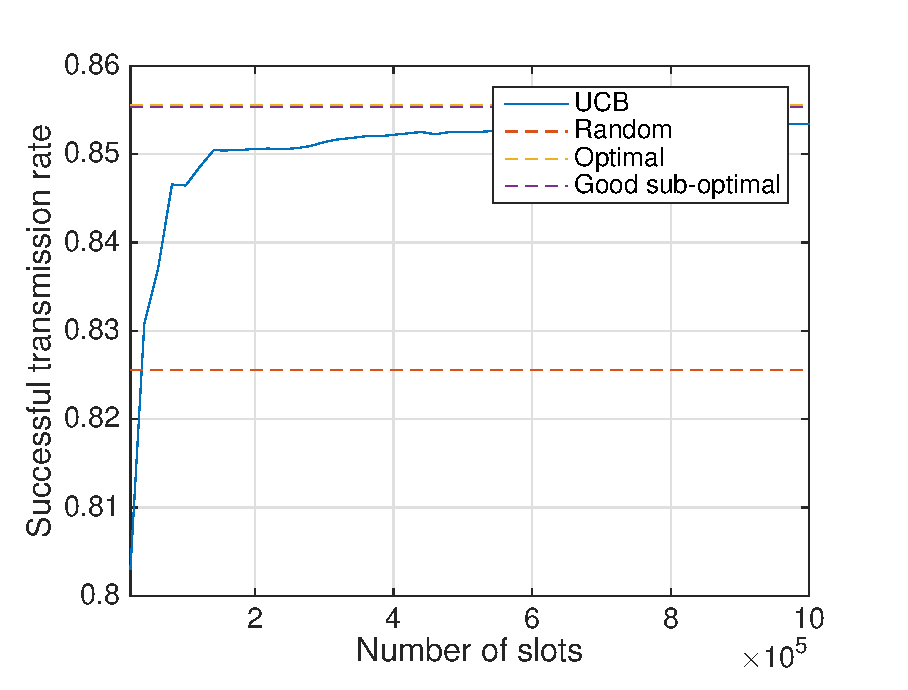
\includegraphics[width=0.47\textwidth]{ch2_50.eps}
    \label{fig:41:ch2_50}}
    %
    \subfloat[][100\% of intelligent devices]{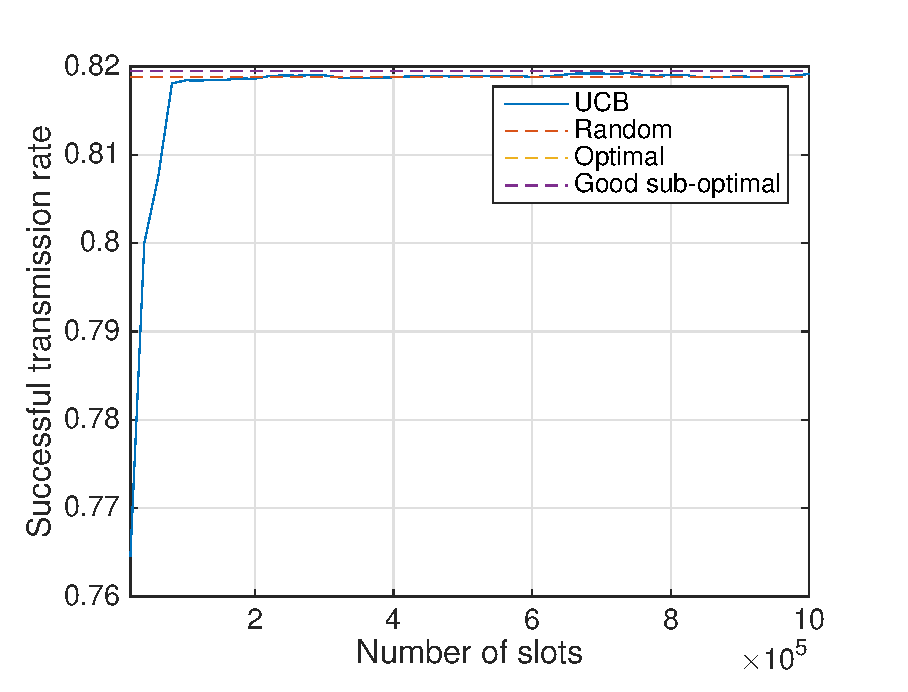
\includegraphics[width=0.47\textwidth]{ch2_100.eps}
    \label{fig:41:ch2_100}}
    \caption{Performance of the UCB bandit algorithm for the special case of uniform repartition of the static devices, when the proportion of intelligent devices in the network increases, from $10\%$ to $100\%$.}
    \label{fig:41:figure4appendix}
\end{figure}

Figure~\ref{fig:41:perf_learning} also shows that learning keeps near-optimal performance even when the proportion of devices becomes large.
Note that when this proportion increases, the assumptions of a stochastic MAB model are clearly violated, and there is no mathematical justification for the efficiency of TS and \UCB{} algorithms.
Hence, it is surprising to have near optimal performance with stochastic MAB algorithms applied to partly or fully dynamic scenarios.


\paragraph{A safety check.}
%
We include another simulation in Figure~\ref{fig:41:figure4appendix}, with a uniform repartition of static devices (\ie, $\forall k, S_k = S/K$), to check that learning approach (here, only \UCB)
also gives interesting gain of performance, and achieve a close-to optimal successful transmission rate.
Except for the limit case of $100\%$ of dynamic devices, which corresponds to Figures~\ref{fig:41:100intelligent} and \ref{fig:41:ch2_100}, where the uniform access performs as well as the optimal oracle solution, the MAB-based approach almost instantly outperforms the baseline.



% \paragraph{Note on the simulation code.}
\paragraph{Reproducibility.}
%
The simulation code used for the experiments in Section~\ref{sub:41:numericalResults} is for MATLAB or GNU Octave,
and it was written in collaboration with Rémi Bonnefoi, in May $2017$.
Instructions to reproduce our experiments are given, and
the code is open-sourced under the MIT License, at
\href{https://Bitbucket.org/scee_ietr/rl_slotted_iot_networks}{\texttt{Bitbucket.org/scee\_ietr/rl\_slotted\_iot\_networks}}.
